\subsection{Assessment and Benchmarking for the EURACE Model}
\label{sec:performance-eurace}
In this section we consider the benchmarking of the full EURACE Model as
described in the other deliverables of the project. Before presenting the
results of the benchmarks it is useful to consider what we are measuring
and why. The goal of most performance analyses is to identify sections
or elements of a program that are taking significant resourses - computational
time - with the aim of optimising these to reduce the total elapsed time
of the simulation. Our purpose is no different from this expect that we
will be considering both serial and parallel performance.

It goes without saying that there is little point assessing the parallel
performance of a code that performing poorly in serial mode. Most of the
components of the code will be executed in both modes although there
may be re-organisation of the control flow. So we start will an analysis
of the serial version of the EURACE Model.

When assessing parallel performance two basic laws influence the developer:
Amdalh's Law and Gustafson's Law. Amdahl's law is a model for the relationship 
between the expected speedup of parallelized implementations of an algorithm 
relative to the serial algorithm, under the assumption that the problem size 
remains the same when parallelized.

Amdahl's law states that if $P$ is the proportion of a program that can be made 
parallel (i.e. benefit from parallelization), and $(1 - P)$ is the proportion 
that cannot be parallelized (remains serial), then the maximum speedup that can 
be achieved by using $N$ processors is
\begin{equation}
	    \frac{1}{(1-P) + \frac{P}{N}}.
\end{equation}
In the limit, as $N$ tends to infinity, the maximum speedup tends to 
${1}/{(1 - P)}$. In practice, performance to price ratio falls rapidly as 
$N$ is increased once there is even a small component of $(1 - P)$.

As an example, if $P$ is $90\%$, then $(1 - P)$ is $10\%$, and the problem 
can be speed up by a maximum of a factor of $10$, no matter how large the 
value of $N$ used. For this reason, it has been often said, parallel computing 
is only useful for either small numbers of processors, or problems with very 
high values of $P$: so-called embarrassingly parallel problems. A great part 
of the craft of parallel programming consists of attempting to reduce the 
component $(1 � P)$ to the smallest possible value.

Fortunately this is not the end of parallel computing. It must be noted that
this was for a \textbf{fixed size} application.  Gustafson's Law paints a
different picture. It states that any sufficiently large problem can be 
efficiently parallelized and the speedup that can be gained is:
\begin{equation}
	S(N) = N - \alpha\cdot(N-1)
\end{equation}
where $N$ is the number of processors, $S$ is the speedup, and $\alpha$ the non-parallelizable part of the process i.e. the serial part.

Gustafson's law addresses the shortcomings of Amdahl's law, which cannot scale to match availability of computing power as the machine size increases. It removes the fixed problem size or fixed computation load on the parallel processors: instead, he proposed a fixed time concept which leads to scaled speed up for larger problem sizes (i.e. weak or soft scaling).

Amdahl's law is based on fixed workload or fixed problem size (i.e. strong or hard scaling). It implies that the sequential part of a program does not change with respect to machine size (i.e, the number of processors). However the parallel part is evenly distributed by $N$ processors.

In both of these formalisations of potential parallel speedup to proportional of serial activity has a significant effect of the potential parallel speedup. However Gustason's Law gives the hope that for
a \textit{sufficiently large} problem parallel performance can be demonstrated.

Although neither of these models completely characterises the exectly situation - it is very difficult to estimate the serial part of a parallel code - it is clear that the serial part has a significant effect on the speed up of any application. So in the assessment of the EURACE Model we will focus on identifying the serial part.

We have developed a number of analysis tools that have allowed us to benchmark any
FLAME model and assess its serial and parallel performance. We have used a number 
of versions of the EURACE Model in this benchmarking - the model has been under 
constant development.




% Serial Performance


\subsection{Serial Performance Analysis}
\label{sec:performance-serial}
This section comprises tables of agent function CPU times recorded with the timer package as the EURACE integrated model has evolved in recent revisions. The code was compiled with debugging and profiling turned on which will have an effect on the absolute timings but not on the proportion of time spent in each routine. 
\begin{table}[h]
	\centering
		\begin{tabular}{|l|c|}\hline
     \bf Agent type & \bf Number of agents\\\hline
\multicolumn{2}{|l|}{\bf National} \\\hline
Government & 1\\
Central\_Bank & 1 \\
Clearinghouse & 1\\
Eurostat & 1\\
IGFirm & 1\\\hline
\multicolumn{2}{|l|}{Regional}\\\hline
Mall &		1\\
Bank & 2\\
Firm &80\\
Household & 1600\\		\hline
\end{tabular}
		\label{table:small-population}
		\caption{Distribution of agent population (small)}
\end{table}
At the start of this analysis (Table \ref{table:r2701}) one \texttt{clearinghouse} agent function took up 72\% of the run time. When this function was profiled with the GNU \texttt{gprof} tool (see Figure \ref{fig:CH_call_graph}) it was found that the time was being taken buy the routine \texttt{newPrice}.
After reviewing the algorithm implemented in \texttt{newPrice} ways were found to improved it in a number of ways which would lead to a halving of the number of calls to \texttt{aggregateDemand} - a core routine of \texttt{newPrice}.  
\begin{table}[h]
	\centering
	{\small\renewcommand{\arraystretch}{1.2}
		\begin{tabular}{|l|r|p{5mm}|l|r|}\hline
		\multicolumn{2}{|c|}{\bf Writing}& &\multicolumn{2}{|c|}{\bf Reading}\\\hline
\bf Message Name & \bf Counts & & \bf Message Name & \bf Counts \\\hline
			order&	57557	&	&order&	2935407 \\
bank\_account\_update	&1551	&	&quality\_price\_info\_1	&13700\\
job\_application	& 666	&	&info\_firm	&7850\\
job\_application2 &	552	&	&accountInterest&	6000\\
order\_status&	337	&	&dividend\_per\_share&	3000\\
accepted\_consumption\_1&	274	&	&bank\_account\_update	&1551\\
consumption\_request\_1&	274	&	&job\_application&	666\\
tax\_payment	&62	&	&vacancies	&666\\
hh\_subsidy\_notification&	60&	&	job\_application2&	552\\
hh\_transfer\_notification&	60&	&	vacancies2&	552\\\hline
		\end{tabular}
		}
		\label{table:message-counts-1}
		\caption{Initial top ten counts of message Reads and Write (population: 1688 agents)}
\end{table}
During a second phase the message counts table - Table~\ref{table:message-counts-1} was generated, This shows the number of message of a particular type that have passed through the system board system. From the timings it is cleat that \texttt{clearinghouse} agent is a serious bottleneck in the simulation. This is re-enforced by Table~\ref{table:message-counts-1} as the \texttt{order} message is the most used message type and this is the primary input message for the \texttt{clearinghouse} agent.

Considerable time was taken in understanding these restuls and various improvements to the algorithms used by the\texttt{clearinghouse} agent were suggested to the modellers.  These improvements were passed on to the modellers and were incroporated into a new version of the code.

Table~\ref{table:message-counts-2} show the message counts after these improvements had been implemented.
\begin{table}[ht]
	\centering
	{\small\renewcommand{\arraystretch}{1.2}
		\begin{tabular}{|l|r|p{5mm}|l|r|}\hline
		\multicolumn{2}{|c|}{\bf Writing}& &\multicolumn{2}{|c|}{\bf Reading}\\\hline
\bf Message Name & \bf Counts & & \bf Message Name & \bf Counts \\\hline
order   &   11929&&quality\_price\_info\_1 &4480 \\
job\_application  &3704&&order & 11929 \\
job\_application2  & 3408&&dividend\_per\_share  & 6400\\
bank\_account\_update&  1681&&job\_application &  3704\\
vaaccepted\_consumption\_1 &  306&&cancies   &  3704\\
consumption\_request\_1   &  306&&job\_application2 & 3408\\
tax\_payment  &  84&&vacancies2    &    3408\\
infoAssetCH  & 81&&accountInterest &  3200\\
hh\_transfer\_notification & 80&&bank\_account\_update &  1681\\
info\_firm    &  80&&info\_firm   &   880\\\hline
		\end{tabular}
		}
		\label{table:message-counts-2}
		\caption{Optimisaed top ten counts of message Reads and Write (population: 1688 agents)}
\end{table}
These changes significantly lowered the time taken by the clearinghouse and this was enough to bring the second placed function in Table \ref{table:r2701} to the top in Table \ref{table:r2723}.

\begin{figure}
{\footnotesize
\begin{verbatim}
 ClearingHouse_receive_orders_and_run (73.5%, called 40 times)
   +----emptyClearing
   +----receiveOrderOnAsset
   | +----setOrder
   | +----isBuyOrder
   | +----addBuyOrder
   | | +----addOrder
   | +----isSellOrder
   | +----addSellOrder
   |   +----setAsSellOrder
   |   | +----getOrderQuantity
   |   +----addOrder
   +----computeAssetPrice (72%, called 2040 times)
   | +----setClearingMechanism
   | +----lastPrice
   | +----runClearing (72%, called 2040 times)
   | | +----buyOrders
   | | +----sellOrders
   | | +----sortOrders
   | | +----newPrice (71.2%, called 2040 times)
   | | | +----aggregateDemand (69.25%, called 4,495,474 times)
   | | | +----aggregateSupply (2%,     called 4,495,474 times)
   | | +----aggregateDemand
   | | +----aggregateSupply
   | | +----ordersMacthing
   | | | +----addOrder
   | | +----rationing
   | |   +----randomize
   | |   +----removeZeroOrders
   | +----addPrice
   | +----addVolume
   +----sendOrderStatus
     +----buyOrders
     +----formedPrice
     +----sellOrders
     \end{verbatim}
     }
\caption{Call graph for \texttt{ClearingHouse$\_$receive$\_$orders$\_$and$\_$run} showing work done in most expensive call path\label{fig:CH_call_graph}}
\end{figure}

\begin{landscape}

\begin{table}[c]
\begin{center}
{\small\renewcommand{\arraystretch}{1.3}
\begin{tabular}{|p{70mm}|p{70mm}|p{70mm}|c|c|}\hline
Function & State from & State to & Time (s) & \% \\ \hline
ClearingHouse$\_$receive$\_$orders$\_$and$\_$run & RECEIVEDINFOSTOCK & COMPUTEDPRICES &  82.81 & 72 \\ \hline
Household$\_$stock$\_$beliefs$\_$formation & CHOOSE$\_$TO$\_$UPDATE$\_$BELIEFS$\_$OR$\_$NOT & BOND$\_$BELIEF$\_$FORMATION &  25.32 & 22 \\ \hline
Household$\_$send$\_$orders & SEND$\_$ORDERS & WAITORDERSTATUS &  2.06 & 1.7 \\ \hline
Household$\_$bond$\_$beliefs$\_$formation & BOND$\_$BELIEF$\_$FORMATION &SEND$\_$ORDERS &  0.44 & 0.38 \\ \hline
Household$\_$rank$\_$and$\_$buy$\_$goods$\_$1 & 09 & 09b &  0.42 & 0.36 \\ \hline
\parbox[t]{6cm}{Firm$\_$read$\_$job$\_$applications$\_$send$\_$\\[-4pt]job$\_$offer$\_$or$\_$rejection} & 03 & 04 &  0.37 & 0.32 \\ \hline
Household$\_$update$\_$its$\_$portfolio & WAITORDERSTATUS & Household$\_$Start$\_$Labour$\_$Role &  0.16 & 0.14 \\ \hline
Household$\_$receive$\_$dividends & 06 & 06b &  0.11 & $<$0.1 \\ \hline
Household$\_$receive$\_$info$\_$interest$\_$from$\_$bank & Household$\_$received$\_$coupons & SELECTSTRATEGY &  0.09 & $<$0.1 \\ \hline
Household$\_$send$\_$account$\_$update & 15 & 16 &  0.09 & $<$0.1 \\ \hline
\end{tabular}
}
\caption{Revision \textbf{2701}, Serial, 40 iterations, small population. Total run time 1:55[m:s]\label{table:r2701}}
\end{center}
\end{table}

\clearpage

\begin{table}[c]
\begin{center}
{\small\renewcommand{\arraystretch}{1.3}
\begin{tabular}{|p{70mm}|p{70mm}|p{70mm}|c|c|}\hline
Function & State from & State to & Time (s) & \% \\ \hline
Household$\_$stock$\_$beliefs$\_$formation & CHOOSE$\_$TO$\_$UPDATE$\_$BELIEFS$\_$OR$\_$NOT & BOND$\_$BELIEF$\_$FORMATION &  245.78 & 61 \\ \hline
Household$\_$send$\_$orders & SEND$\_$ORDERS & WAITORDERSTATUS &  46.44 & 11 \\ \hline
ClearingHouse$\_$receive$\_$orders$\_$and$\_$run & RECEIVEDINFOSTOCK & COMPUTEDPRICES &  41.76 & 10 \\ \hline
Household$\_$bond$\_$beliefs$\_$formation & BOND$\_$BELIEF$\_$FORMATION &SEND$\_$ORDERS &  4.98 & 1.2 \\ \hline
Household$\_$update$\_$its$\_$portfolio & WAITORDERSTATUS & Household$\_$Start$\_$Labour$\_$Role &  1.48 & 0.3 \\ \hline
Household$\_$rank$\_$and$\_$buy$\_$goods$\_$1 & 09 & 09b &  1.04 & 0.28 \\ \hline
Household$\_$rank$\_$and$\_$buy$\_$goods$\_$2 & 11 & 12 &  0.9 & 0.22 \\ \hline
Household$\_$receive$\_$dividends & 06 & 06b &  0.8 & 0.20 \\ \hline
Household$\_$receive$\_$info$\_$interest$\_$from$\_$bank & Household$\_$received$\_$coupons & SELECTSTRATEGY &  0.79 & 0.20 \\ \hline
\parbox[t]{6cm}{Firm$\_$read$\_$job$\_$applications$\_$send$\_$\\[-4pt]job$\_$offer$\_$or$\_$rejection}  & 03 & 04 &  0.62 & 0.15 \\ \hline
\end{tabular}
}
\caption{Revision \textbf{2723}, Serial, 240 iterations, small population. Total run time 6:42[m:s]\label{table:r2723}}
\end{center}
\end{table}
\clearpage

\begin{table}[c]
\begin{center}
{\small\renewcommand{\arraystretch}{1.3}
\begin{tabular}{|p{70mm}|p{70mm}|p{70mm}|c|c|}\hline
Function & State from & State to & Time (s) & \% \\ \hline
Household$\_$send$\_$orders & SEND$\_$ORDERS & WAITORDERSTATUS &  63.8842 & 33.3 \\ \hline
ClearingHouse$\_$receive$\_$orders$\_$and$\_$run & RECEIVEDINFOSTOCK & COMPUTEDPRICES &  59.7536 & 31.1 \\ \hline
Household$\_$stock$\_$beliefs$\_$formation & CHOOSE$\_$TO$\_$UPDATE$\_$BELIEFS$\_$OR$\_$NOT & BOND$\_$BELIEF$\_$FORMATION &   8.82473 & 4.6 \\ \hline
Household$\_$rank$\_$and$\_$buy$\_$goods$\_$1 & 09 & 09b &   5.23093 & 2.7 \\ \hline
\parbox[t]{6cm}{Firm$\_$read$\_$job$\_$applications$\_$send$\_$job$\_$\\[-4pt]offer$\_$or$\_$rejection} & 03 & 04 &   1.41734 & 0.7 \\ \hline
Household$\_$receive$\_$dividends & 06 & 06b &   1.38099 & 0.7 \\ \hline
\parbox[t]{6cm}{Household$\_$receive$\_$info$\_$interest$\_$\\[-4pt]from$\_$bank} & Household$\_$received$\_$coupons & SELECTSTRATEGY &   1.14297 & 0.6 \\ \hline
Household$\_$update$\_$its$\_$portfolio & WAITORDERSTATUS & Household$\_$Start$\_$Labour$\_$Role &   1.11446 & 0.6 \\ \hline
Household$\_$receive$\_$data & Household$\_$Start$\_$Policy$\_$Data & Household$\_$Start$\_$Financial$\_$Market$\_$Role &   0.619365 & 0.3 \\ \hline
Household$\_$send$\_$account$\_$update & 15 & 16 &   0.607822 & 0.3 \\ \hline
\end{tabular}
}
\caption{Revision \textbf{2772}, Serial, 240 iterations, small population. Total run time 3:12[m:s]}
\end{center}
\end{table}

\clearpage
\begin{table}[c]
\begin{center}
{\small\renewcommand{\arraystretch}{1.3}
\begin{tabular}{|p{70mm}|p{70mm}|p{70mm}|c|c|}\hline
Function & State from & State to & Time (s) & \% \\ \hline
Household$\_$send$\_$orders & SEND$\_$ORDERS & WAITORDERSTATUS &  77.95 & 37.5 \\ \hline
ClearingHouse$\_$receive$\_$orders$\_$and$\_$run & RECEIVEDINFOSTOCK & COMPUTEDPRICES &   54.51 & 26.2 \\ \hline
Household$\_$stock$\_$beliefs$\_$formation & \parbox[t]{6cm}{CHOOSE$\_$TO$\_$UPDATE$\_$BELIEFS$\_$\\[-4pt]OR$\_$NOT} & BOND$\_$BELIEF$\_$FORMATION &   9.83 & 4.7 \\ \hline
Household$\_$rank$\_$and$\_$buy$\_$goods$\_$1 & 09 & 09b &   3.91 & 1.9 \\ \hline
Household$\_$receive$\_$dividends & 06 & 06b &   1.47 & 0.7 \\ \hline
Household$\_$update$\_$its$\_$portfolio & WAITORDERSTATUS & Household$\_$Start$\_$Labour$\_$Role &   1.34 & 0.6 \\ \hline
\parbox[t]{6cm}{Firm$\_$read$\_$job$\_$applications$\_$send$\_$job$\_$\\[-4pt]offer$\_$or$\_$rejection} & 03 & 04 &   0.98 & 0.5 \\ \hline
Household$\_$select$\_$strategy & SELECTSTRATEGY & CHOOSE$\_$TO$\_$UPDATE$\_$BELIEFS$\_$OR$\_$NOT &   0.8 & 0.4 \\ \hline
\parbox[t]{6cm}{Household$\_$receive$\_$info$\_$interest$\_$\\[-4pt]from$\_$bank} & Household$\_$received$\_$coupons & REVISE$\_$PORTFOLIO &   0.76 & 0.4 \\ \hline
Household$\_$send$\_$account$\_$update & 15 & 16 &  0.64 & 0.3 \\ \hline
\end{tabular}
}
\caption{Revision \textbf{2802}, Serial, 240 iterations, small population. Total run time 3:28[m:s]}
\end{center}
\end{table}

\end{landscape}
This types of iterative analysis and optimisation has been used to improve the performance the EURACE model.


%Parallel Performance

\subsection{Parallel Performance Analysis}
\label{sec:performance-parallel}
In Appendix~\ref{app:initial-benchmarks} the results from the initial parallel benchmarks are described. These models are characterised in Tabel~\ref{table:initial-models}. In general the results showed promising parallel speedup using up to 40 processors.
\begin{table}[ht]
 \centering
  \begin{tabular}{l|ccc}
  Model     & Agents & Messages & Population   \\\hline
   Circles     &   1    &   1      &  10$^5$    \\
   C@S       &   3    &   9      &  124,000 \\
   Labour Market &   4    &   10     &  110,101 \\ 
   Bielefeld     &   4    &   29     &  43100     \\\hline
   \end{tabular}
   \caption{Details of Initial Benchmark Models}
   \label{table:initial-models}
 \end{table}
However as the number of message used by a model - as in the case of the Bielefeld model - some irratic behaviour was observed. Table~\ref{table:eurace-model} gives the characteristics of the full integrated EURACE Model. It is most important to note that the number of message types is 62 -  a great many more than previous models. 
\begin{table}[ht]
 \centering
  \begin{tabular}{l|ccc}
  Model     & Agents & Messages & Population   \\\hline
  EURACE     &   9    &   62      &  ~30,000 \\
  \end{tabular}
  \caption{Details of the EURACE Model}
  \label{table:eurace-model}
 \end{table}

Analysis of parallel performance includes profiling the agent functions as for the serial case but also investigating how the EURACE application performs as the number of processes is increased for a fixed initial population. The profiling of agent functions is shown in Tables \ref{table:r2754_0} and \ref{table:r2754_1} and it is clear that the clearinghouse agent function for finding the correct market price for assets is dominant. Not only that; because there is only one clearinghouse it is a serious \textbf{serial bottleneck}. All agents have to wait for it to complete its calculations before they can carry on. The household function for sending orders is not a bottleneck since the agents are distributed round the processes by FLAME.

Although FLAME makes great efforts to maximise the time available to synchronise the message boards, as explained in Section~\label{sec:performance-flame}, this will only have an effect if the function in question has potential parallel tasks. Unfortunately the Clearing House, and particular when computing the correct market price for assets, requires asset and order information from all Firm and Household agents before it is able to perform the calculation. This generates a serial bottleneck which will have a serious effect on performance. This is reflected in the timings in Table~\ref{table:r2754_1} - the Clear House is top of the list. All other agents - and processors - much wait until the Clear House completes its work - which is around 35\% of the runtime.

Although this is a serious problem in terms of performance it is still possible to perform runs of the EURACE model with larger populations. Using a 16 region model with 26948 agents runs have been carried out on large parallel machines available to STFC, namely HAPU, NW-Grid and Hector. Details of these machines can be found in Appendix \ref{app:parallel-systems}. 



\begin{landscape}
\begin{table}[c]
\begin{center}
{\small\renewcommand{\arraystretch}{1.3}
\begin{tabular}{|p{70mm}|p{70mm}|p{70mm}|c|c|}\hline
Function & State from & State to & Time (s) & \% \\ \hline
Household$\_$send$\_$orders & SEND$\_$ORDERS & WAITORDERSTATUS &   2083.3 & 14.2 \\ \hline
Household$\_$stock$\_$beliefs$\_$formation & CHOOSE$\_$TO$\_$UPDATE$\_$BELIEFS$\_$OR$\_$NOT & BOND$\_$BELIEF$\_$FORMATION &   211.144 & 1.4 \\ \hline
order &  &  &   137.024 & 0.9 \\ \hline
Household$\_$receive$\_$dividends & 06 & 06b &   104.891 & 0.7 \\ \hline
Household$\_$receive$\_$data & Household$\_$Start$\_$Policy$\_$Data & Household$\_$Start$\_$Financial$\_$Market$\_$Role &   43.6602 & 0.3 \\ \hline
Household$\_$receive$\_$info$\_$interest$\_$from$\_$bank & Household$\_$received$\_$coupons & SELECTSTRATEGY &   37.1621 & 0.3 \\ \hline
Household$\_$update$\_$its$\_$portfolio & WAITORDERSTATUS & Household$\_$Start$\_$Labour$\_$Role &   34.5611 & 0.2 \\ \hline
Firm$\_$read$\_$stock$\_$transactions & 0003 & End$\_$Firm$\_$Financial$\_$Role &   17.7424 & 0.1 \\ \hline
Household$\_$rank$\_$and$\_$buy$\_$goods$\_$1 & 09 & 09b &   16.1013 & 0.1 \\ \hline
Household$\_$send$\_$account$\_$update & 15 & 16 &   16.049 & 0.1 \\ \hline
\end{tabular}
}
\caption{Revision \textbf{2754}, Parallel, 240 iterations, 16 region population. Total run time 244:25[m:s]. Node 0\label{table:r2754_0}}
\end{center}
\end{table}

\clearpage
\begin{table}[c]
\begin{center}
{\footnotesize\renewcommand{\arraystretch}{1.3}
\begin{tabular}{|p{70mm}|p{70mm}|p{70mm}|c|c|}\hline
Function & State from & State to & Time (s) & \% \\ \hline
ClearingHouse$\_$receive$\_$orders$\_$and$\_$run & RECEIVEDINFOSTOCK & COMPUTEDPRICES &   5125.29 & 35.0 \\ \hline
Household$\_$send$\_$orders & SEND$\_$ORDERS & WAITORDERSTATUS &   2067.41 & 14.1 \\ \hline
Household$\_$stock$\_$beliefs$\_$formation & CHOOSE$\_$TO$\_$UPDATE$\_$BELIEFS$\_$OR$\_$NOT & BOND$\_$BELIEF$\_$FORMATION &  222.105 & 1.5 \\ \hline
Household$\_$receive$\_$dividends & 06 & 06b &   104.267 & 0.7 \\ \hline
order &  &  &   75.312 & 0.5 \\ \hline
Household$\_$receive$\_$data & Household$\_$Start$\_$Policy$\_$Data & Household$\_$Start$\_$Financial$\_$Market$\_$Role &   43.5033 & 0.3 \\ \hline
Household$\_$receive$\_$info$\_$interest$\_$from$\_$bank & Household$\_$received$\_$coupons & SELECTSTRATEGY &   37.0695 & 0.3 \\ \hline
Household$\_$update$\_$its$\_$portfolio & WAITORDERSTATUS & Household$\_$Start$\_$Labour$\_$Role &   34.4162 & 0.2 \\ \hline
Household$\_$rank$\_$and$\_$buy$\_$goods$\_$1 & 09 & 09b &   16.4965 & 0.1 \\ \hline
Firm$\_$read$\_$stock$\_$transactions & 0003 & End$\_$Firm$\_$Financial$\_$Role &   15.9953 & 0.1 \\ \hline
\end{tabular}
}\caption{Revision \textbf{2754}, Parallel, 240 iterations, 16 region population. Total run time 244:25[m:s]. Node 1\label{table:r2754_1}}
\end{center}
\end{table}

\end{landscape}

The graph of average iteration time (seconds) against number of processes is shown in Figure \ref{fig:speedup}. 	Some interesting features can be seen in this graph: it can be observed that Hector shows generally good speedup, the NW-Grid machine shows a little but HAPU shows some seriously eratic behaviour. The iteration times are given in Table \ref{table:speedup}.

\begin{figure}[ht]
 \centering
  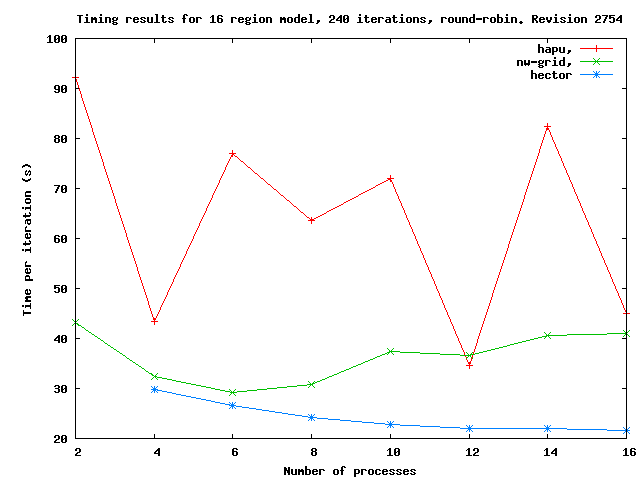
\includegraphics[width=330pt]{speedup.png}
 \caption{Average iteration times (s) 240 iterations of 16 region EURACE model}
 \label{fig:speedup}
\end{figure}

\begin{table}[ht]
\begin{center}
\begin{tabular}{|l|l|l|l|} \hline
Num processes & HAPU & NW-Grid & Hector \\ \hline
2   & 92.3 & 43.2 & - \\ \hline
4   & 43.3 & 32.4 & 29.8 \\ \hline
6   & 76.9 & 29.3 & 26.6 \\ \hline
8   & 63.6 & 30.8 & 24.1 \\ \hline
10  & 72.1 & 37.3 & 22.9 \\ \hline
12  & 34.6 & 36.5 & 22.0 \\ \hline
14  & 82.5 & 40.5 & 22.1 \\ \hline
16  & 45.0 & 41.0 & 21.7 \\ \hline
\end{tabular}
\caption{Average iteration times for 16 region EURACE model}
\label{table:speedup}
\end{center}
\end{table}

Although the HECToR and NW-GRID results show some parallel performance it is disappointing. The HAPU results show some very strange behaviour which can only really be explained by defficiencies in the EURACE Model algorithms. During the assessment of the model it has been shown to be very sensitive to changes in parameter values: sometimes failing with zero divides but more often or not terminating in an infinite loop. The model in very
complex and it is very difficult to debug. Programming conventions and testing proceedures - as defined in the project - have help elliminate many problems but as one might expect there will be residual bugs.

Throughout the assessment critical algorithms have been review and improvements made but there are still many processes that are not particularly robust. Given the very complex interactions between agents one could not expect every computational situation to have been covered. Only significant more testing and detailed evaluation and detailed assessment of the EURACE algorithm will lead to a robust simulator.

The results from running the EURACE Model in parallel have been very disappointing. The stability of the model has been very poor and as are these intial results.

As mentioned earlier the EURACE Model is being continually improve and developed so the results in this report are only a snapshot of the status at the time of writing.